\section{图\&表}

\subsection{图}

\subsubsection{单图}

单行单图如图 \ref{fig:demo} 所示

\begin{figure}[htbp]
    \centering
    
\includegraphics[width=0.9\linewidth]{demo.png}
    \caption{demo}
    \label{fig:demo}
\end{figure}

\subsubsection{多图}

单行多图如图 \ref{fig:login}, \ref{fig:reg} 所示

\begin{figure}[H]
    \begin{minipage}[t]{0.49\linewidth}
        \centering
        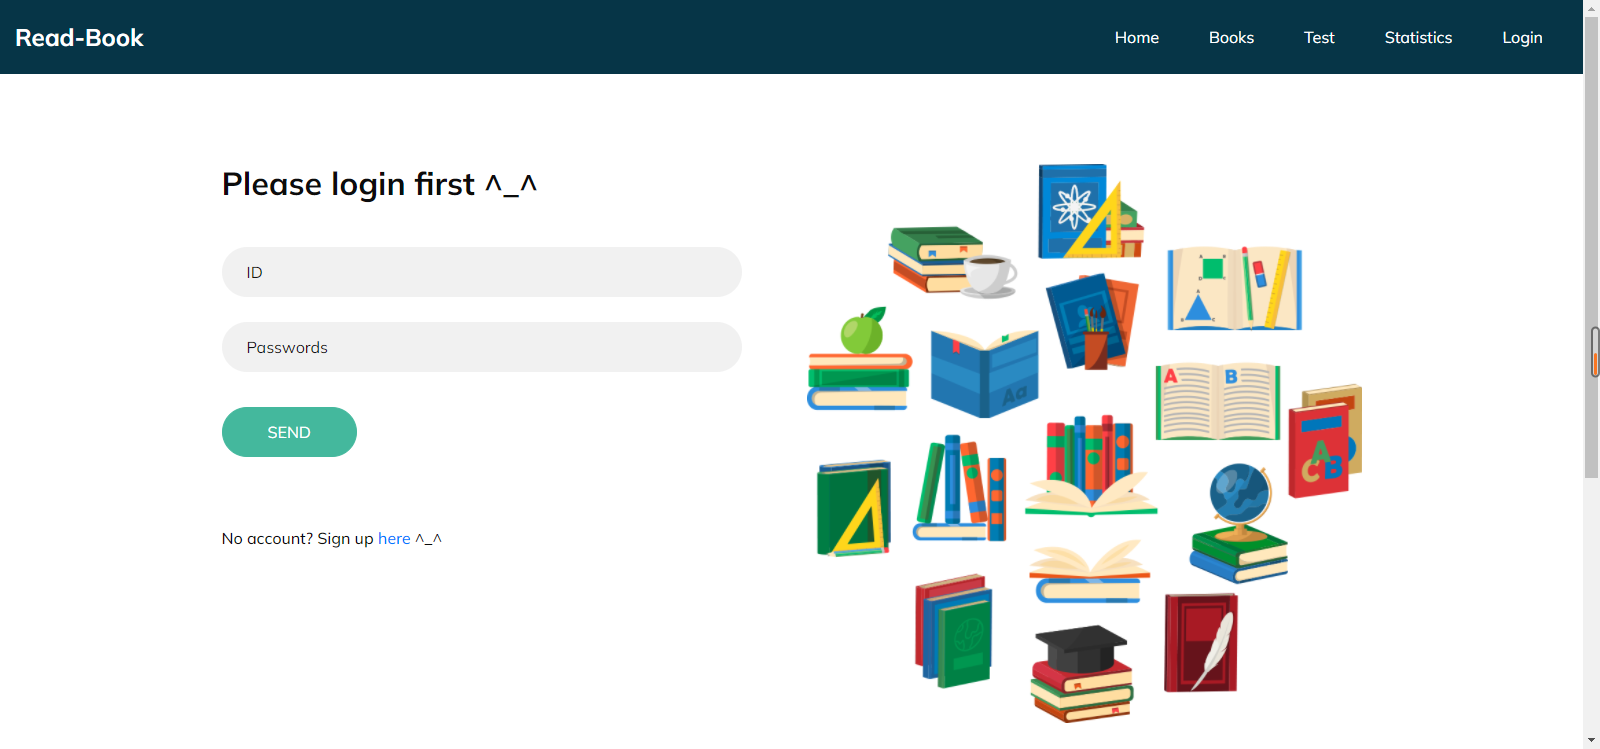
\includegraphics[width=0.95\columnwidth]{login.png}
        \caption{Login}\label{fig:login}
    \end{minipage}
    \begin{minipage}[t]{0.49\linewidth}
        \centering
        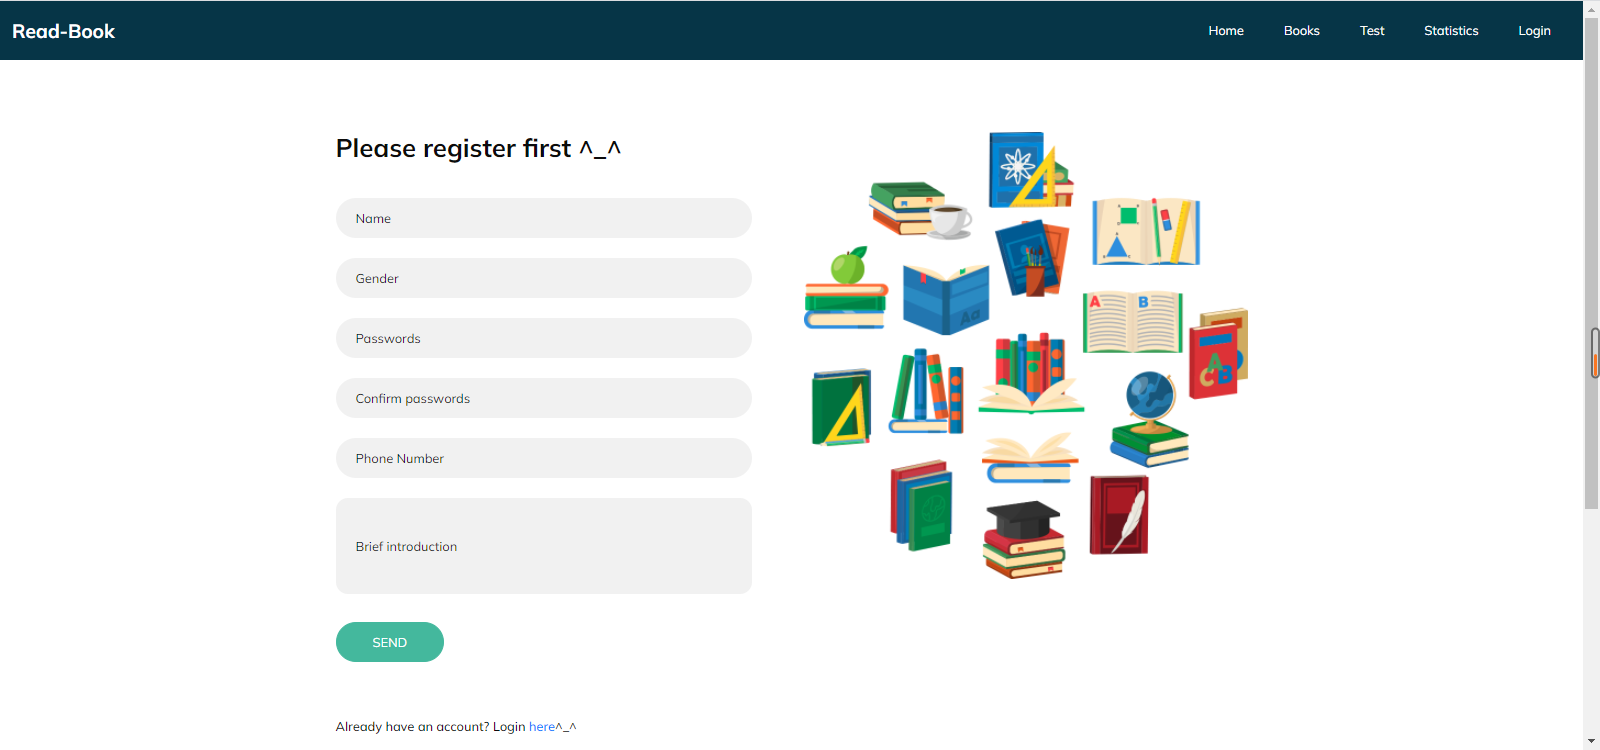
\includegraphics[width=0.95\columnwidth]{reg.png}
        \caption{Register}\label{fig:reg}
    \end{minipage}
\end{figure}

\newpage

\subsection{表}
\subsubsection{三线表}

\begin{table}[h]
    \caption{demo}
    \label{tab:1}
    \xiaowu
    \centering
    \begin{tabular}{c c c c}
        \hline
        \textbf{Name}        & \textbf{Value} \\
        \hline

        ADF Statistic        & -0.501         \\
        p-value              & 0.892          \\
        Critical Values:1\%  & -3.493         \\
        Critical Values:5\%  & -2.892         \\
        Critical Values:10\% & -2.583         \\
        \hline
    \end{tabular}
\end{table}
\subsubsection{跨页表}

\begin{longtable}{>{\sihao}c >{\wuhao }l >{\sihao}c >{\wuhao }l}
    \caption{在线学习标准}                                                                                                                                                                                         \\
    \toprule
    \textbf{\wuhao 标准类型}                                & \multicolumn{1}{c}{\wuhao  \textbf{标准内容}} & \textbf{\wuhao 标准类型}                             & \multicolumn{1}{c}{\wuhao  \textbf{标准内容}} \\
    \midrule
    \endhead

    \bottomrule
    \endfoot
    \bottomrule
    \endlastfoot

    \multirow{10}{*}{\rotatebox[origin=c]{90}{1. 平台}}     & 1. MOOC                                       & \multirow{11}{*}{\rotatebox[origin=c]{90}{3. 评估} } & 20. 电子学习人格化                            \\
                                                            & 2. 移动学习系统                               &                                                      & 21. 电子学习体验                              \\
                                                            & 3. 微软Teams                                  &                                                      & 22. 学生集中程度                              \\
                                                            & 4. MoodleRec                                  &                                                      & 23. 在线教学的有效性                          \\
                                                            & 5. Web 2.0                                    &                                                      & 24. 电子学习的成效                            \\
                                                            & 6. 移动学习平台                               &                                                      & 25. 组织、教学、技术                          \\
                                                            & 7. 移动教学平台                               &                                                      & 26. 感知满意度                                \\
                                                            & 8. 混合型教学平台                             &                                                      & 27. 感知有用性                                \\
                                                            & 9. 在线教学平台                               &                                                      & 28. 学生的看法                                \\
                                                            & 10. 教学管理系统                              &                                                      & 29. 学生准备                                  \\
    \multirow{10}{*}{\rotatebox[origin=c]{90}{2. 评估标准}} & 1. 5维评价模型                                &                                                      & 30. 学习成绩                                  \\
                                                            & 2. Kirkpatrick模型                            & \multirow{8}{*}{\rotatebox[origin=c]{90}{4. 模型}}   & 1.卷积神经网络                                \\
                                                            & 3. 系统实用性量表                             &                                                      & 2. BP 神经网络                                \\
                                                            & 4. Technological Acceptance (TAM)             &                                                      & 3. 互联网 +                                   \\
                                                            & 5. SWOT 分析                                  &                                                      & 4. 自主学习                                   \\
                                                            & 6. 平衡计分卡 (BSC)                           &                                                      & 5. 紧急远程教育                               \\
                                                            & 7. 计划行为理论 (TPB)                         &                                                      & 6. 紧急远程教学                               \\
                                                            & 8. 预期确认模型 (ECM)                         &                                                      & 7. Personal Zed E-learning                    \\
                                                            & 9. 心流理论                                   &                                                      & 8. 紧急远程学习 (ERL)                         \\
                                                            & 10. E-Learning System Model                   & \multirow{5}{*}{\rotatebox[origin=c]{90}{5. 方法}}   & 1. 微课教学方法                               \\
                                                            & 1. 服务质量                                   &                                                      & 2. 翻转课堂                                   \\
                                                            & 2. 学习态度                                   &                                                      & 3. 虚拟教室                                   \\
                                                            & 3. 学习过程                                   &                                                      & 4. 脑电图 (EEG)                               \\
                                                            & 4. 学习效果                                   &                                                      & 5. 心率变化 (HRV)                             \\
                                                            & 5. 学习投入                                   &                                                      & 1. 在线教学不均衡                             \\
                                                            & 6. 用户满意度                                 &                                                      & 2. 缺乏理性自省                               \\
                                                            & 7. 实用性                                     &                                                      & 3. 教育科目的价值被削弱                       \\
    \multirow{12}{*}{\rotatebox[origin=c]{90}{3. 评估}}     & 8. 电子学习的实用性                           & \multirow{8}{*}{\rotatebox[origin=c]{90}{6. 问题}}   & 4. 社会隔离                                   \\
                                                            & 9. 性别                                       &                                                      & 5. 教学环境                                   \\
                                                            & 10. 采用技术                                  &                                                      & 6. 课堂教学                                   \\
                                                            & 11. 教学质量                                  &                                                      & 7. 学生需求                                   \\
                                                            & 12. 学习成绩                                  &                                                      & 8. 使用数字工具的准备情况                     \\
                                                            & 13. 技术使用                                  &                                                      & 9. 缺乏能力                                   \\
                                                            & 14. 学习热情                                  &                                                      & 10. 消极表现                                  \\
                                                            & 15. 学习兴趣                                  &                                                      & 11. 缺乏经验                                  \\
                                                            & 16. 学生和教育工作者的态度                    & \multirow{3}{*}{\rotatebox[origin=c]{90}{7. 趋势}}   & 1. 社交网络的使用                             \\
                                                            & 17. 认知能力发展                              &                                                      & 2. 语义网                                     \\
                                                            & 18. 教育环境                                  &                                                      & 3. 智能技术                                   \\
                                                            & 19. 智力活动                                  &                                                      &

    \label{tab:tech}
\end{longtable}